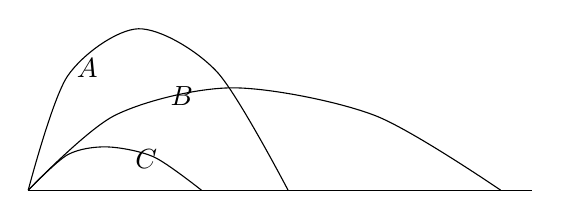
\begin{tikzpicture}[scale=1.0]
  % ground
  \draw (0,0) -- (6.4,0);
  % trajectory A (tall, narrow)
  \draw plot[smooth] coordinates {(0,0) (0.5,1.45) (1.4,2.05) (2.4,1.5) (3.3,0)};
  % trajectory B (medium, wide)
  \draw plot[smooth] coordinates {(0,0) (1.1,0.95) (2.6,1.3) (4.4,0.95) (6,0)};
  % trajectory C (small, short)
  \draw plot[smooth] coordinates {(0,0) (0.5,0.45) (1.0,0.55) (1.6,0.42) (2.2,0)};
  % labels
  \node at (0.75,1.55) {$A$};
  \node at (1.95,1.2) {$B$};
  \node at (1.5,0.4) {$C$};
\end{tikzpicture}
